\section{L'environnement du développeur}
\label{sec:environnement}

\subsection{L'éditeur}
\label{subsec:editeur}

\begin{frame}
    \frametitle{Environnement de développement intégré (IDE)}

    Un environnement de développement intégré est une application logicielle
    qui fournit des \emph{fonctionnalités complètes pour le développement de logiciels}.

    Les IDE sont conçus pour \textbf{maximiser la productivité des programmeurs}
    en fournissant des composants étroitement intégrés qui fournissent de nombreuses fonctionnalités :
    \begin{itemize}
        \item Edition de texte ;
        \item Vérification de syntaxe ;
        \item Gestion de version ;
        \item Compilation ;
        \item Gestion des tests ;
        \item Débogage de logiciel ;
        \item \ldots
    \end{itemize}
\end{frame}

\begin{frame}
    \frametitle{Une usine à gaz\ldots}
    \centering
    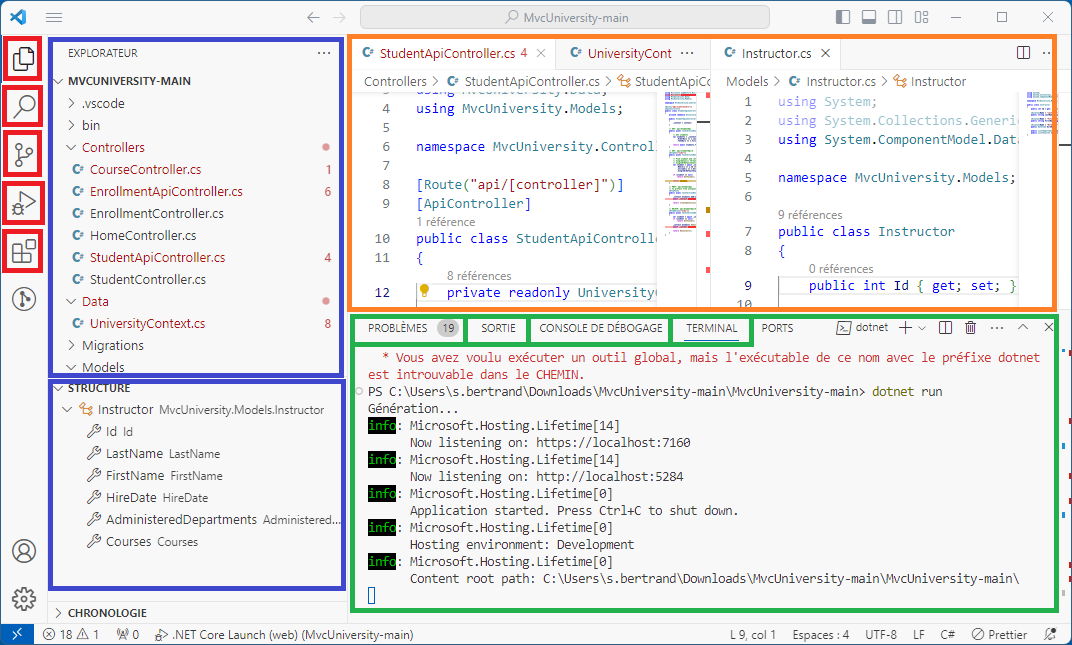
\includegraphics[height=0.5\linewidth]{figures/environnement/vscode}
\end{frame}

\begin{frame}
    \frametitle{Définition et références}
    \centering
    \Huge
    \textbf{CTRL + CLIC}

    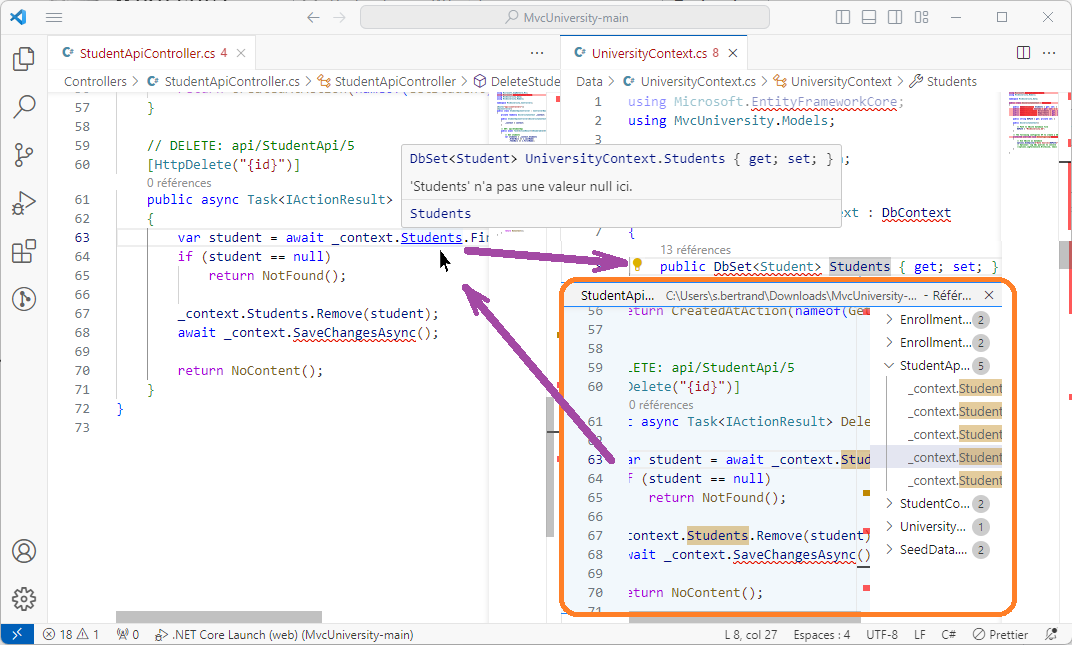
\includegraphics[height=0.4\linewidth]{figures/environnement/controle-clic}
\end{frame}

\begin{frame}
    \frametitle{Recherche}
    \centering
    \Huge
    \textbf{CTRL + (MAJ) + F}

    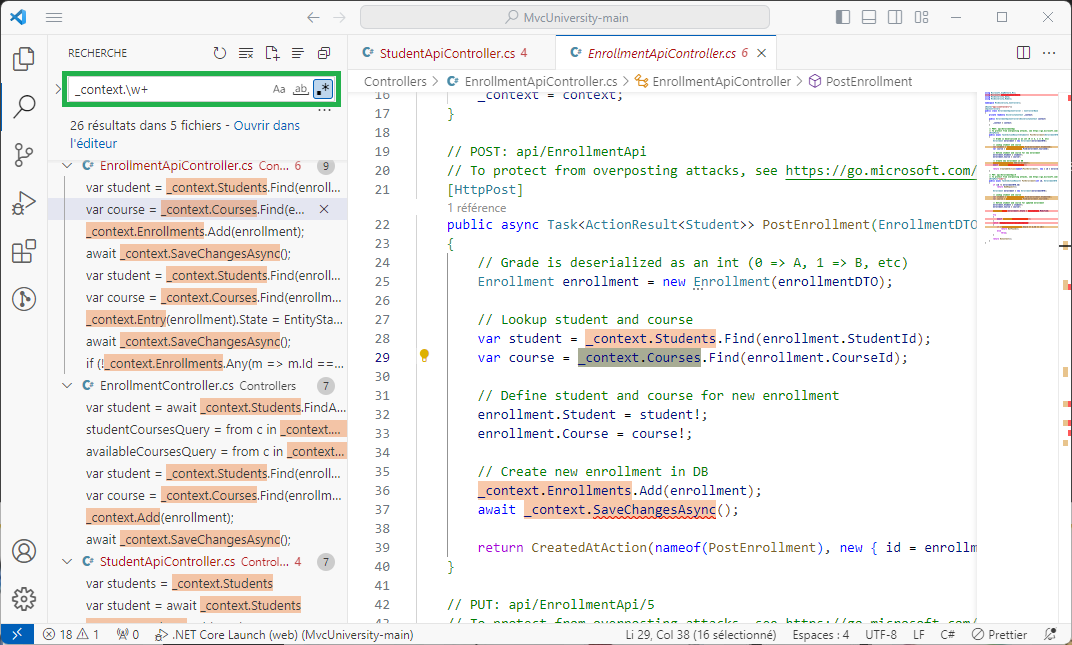
\includegraphics[height=0.4\linewidth]{figures/environnement/rechercher}
\end{frame}

\begin{frame}[fragile]
    \frametitle{Les expressions régulières}
    \begin{columns}
        \begin{column}{0.7\textwidth}
            \begin{itemize}
                \item \verb|[A-Z]\w+| : n'importe quel mot qui commence par une majuscule ;
                \item \verb|.*| : n'importe quelle suite de caractère (sauf \verb|\n| et \verb|\r|) ;
                \item \verb|a*\w+| : \verb|a*| ne sert à rien ;
                \item \verb|[+-]?(\d*[.])?\d+| : Nombre à virgule flottante.
            \end{itemize}
        \end{column}
        \begin{column}{0.3\textwidth}
            \centering

            \qrcode[height=70pt]{https://regexr.com/}
        \end{column}
    \end{columns}
\end{frame}

\begin{frame}
    \frametitle{Remplacer à l'aide des expressions régulières}
    \centering
    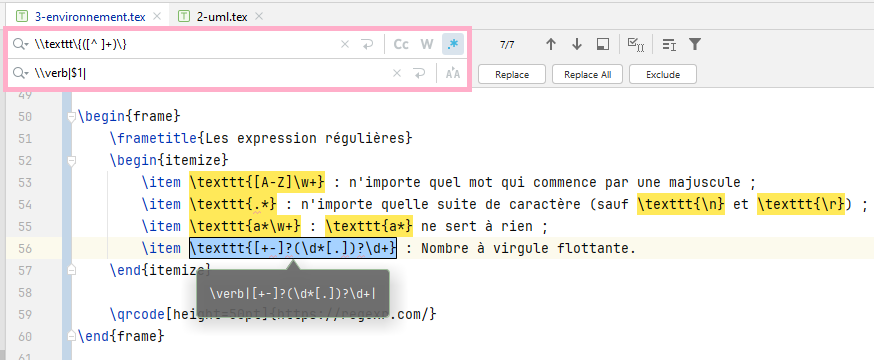
\includegraphics[height=0.4\linewidth]{figures/environnement/remplacer}
\end{frame}

\begin{frame}
    \frametitle{Renommer un élément de programme}
    \centering
    \Huge
    \textbf{F2}

    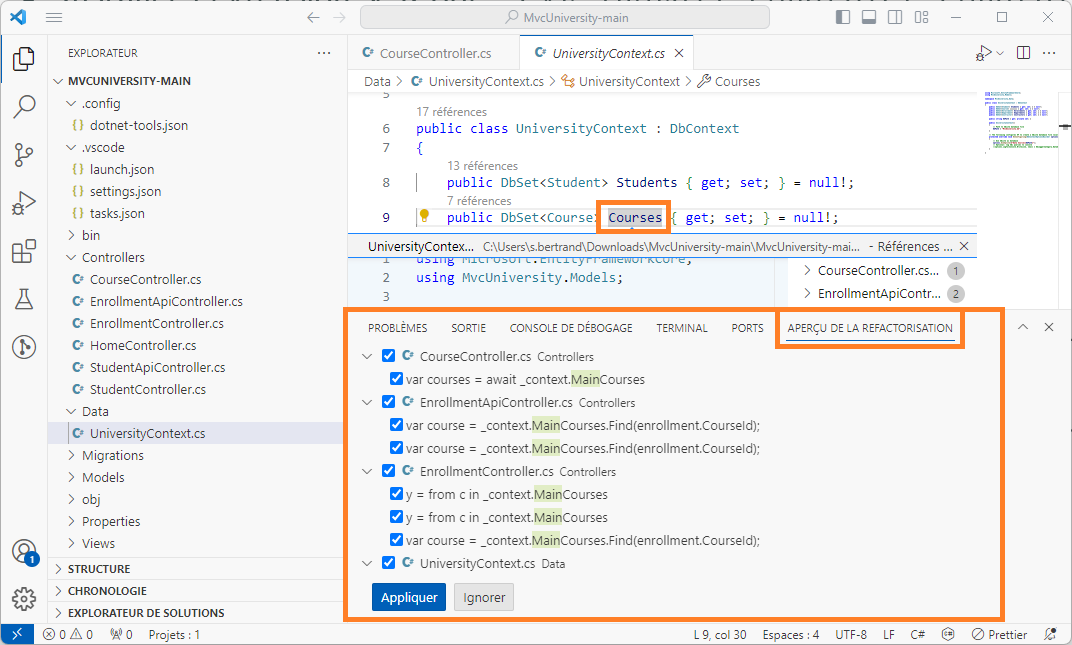
\includegraphics[height=0.4\linewidth]{figures/environnement/renommer}
\end{frame}

\begin{frame}
    \frametitle{Refactoriser}
    \centering
    \Huge\textbf{CTRL + MAJ + R}\\
    \normalsize Installer l'extension VSCode : \texttt{ext install ms-dotnettools.csdevkit} (CTRL+P)

    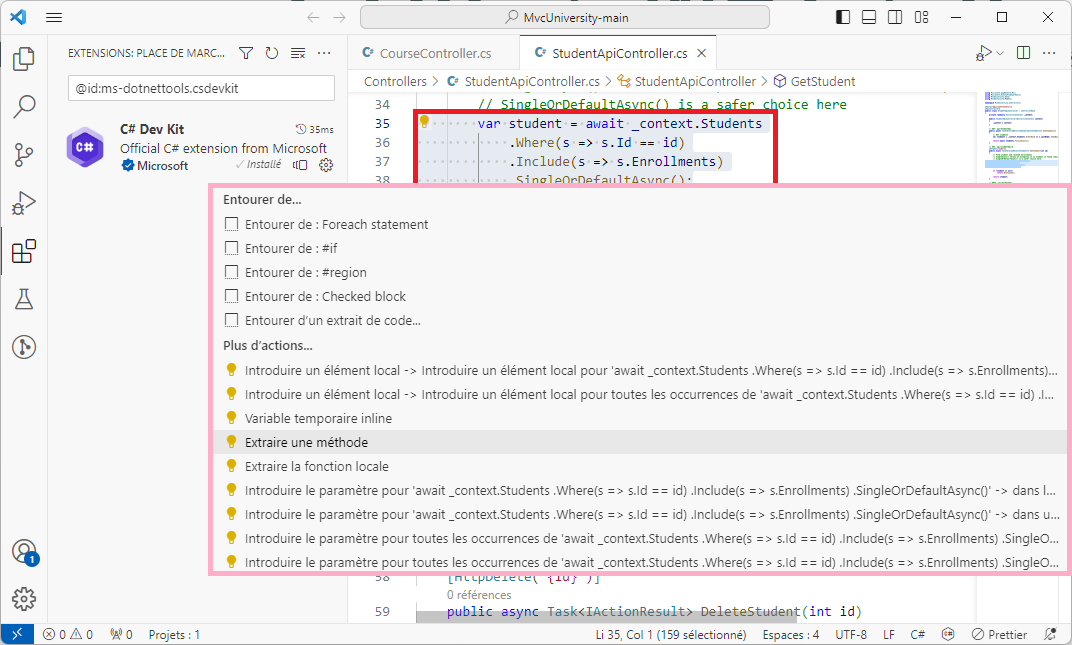
\includegraphics[height=0.35\linewidth]{figures/environnement/refactoriser}
\end{frame}

\begin{frame}
    \frametitle{Editer plusieurs ligne à la fois}
    \centering
    \Huge\textbf{ALT + CLIC}

    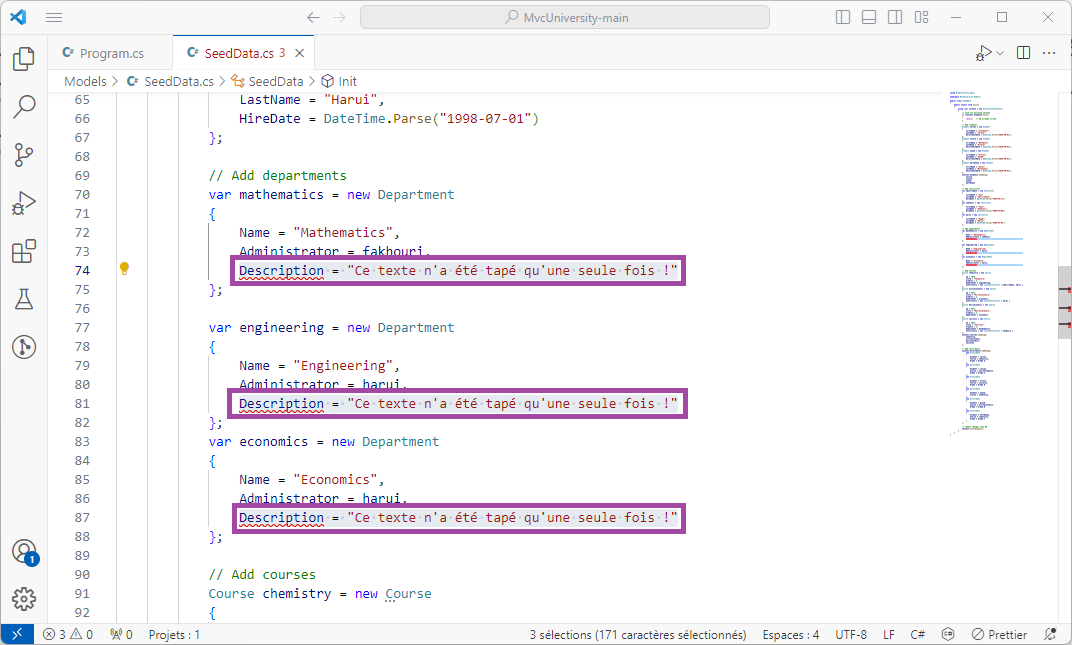
\includegraphics[height=0.4\linewidth]{figures/environnement/multi-edition}
\end{frame}

\begin{frame}
    \frametitle{Présenter le code source}
    \centering
    \Huge
    \textbf{CTRL + ALT + F}

    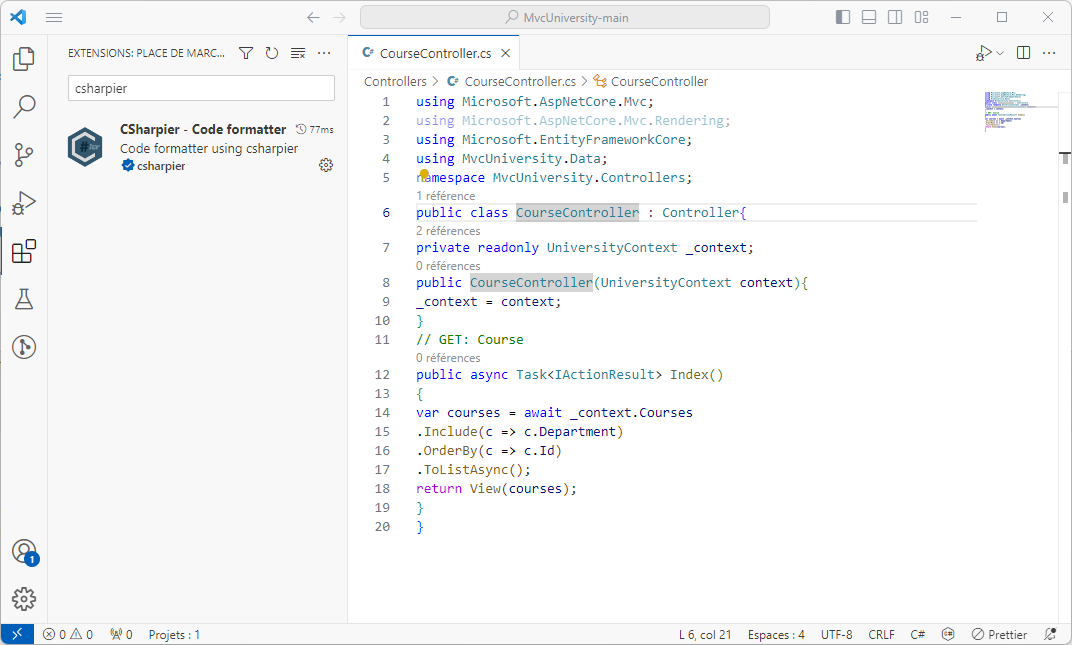
\includegraphics[height=0.4\linewidth]{figures/environnement/mise-en-forme}
\end{frame}

\begin{frame}[fragile]
    \frametitle{Installer CSharpier}
    \centering
    \begin{itemize}
        \item Installer l'outil DotNet : \texttt{dotnet tool install csharpier -g}
        \item Installer l'extension VSCode : \texttt{ext install csharpier.csharpier-vscode} (CTRL+P)
        \item Configurer en tant que formateur par défaut (Paramètres)
        \item Activer \enquote{Format On Save}
        \item Editer le fichier \texttt{/.vscode/settings.json}):
    \end{itemize}

    \begin{verbatim}
    "editor.defaultFormatter": "csharpier.csharpier-vscode",
    "[csharp]": {
        "editor.defaultFormatter": "csharpier.csharpier-vscode"
    },
    \end{verbatim}
\end{frame}

\begin{frame}
    \frametitle{Une commande pour les gouverner toutes}
    \centering
    \Huge
    \textbf{CTRL + MAJ + P}

    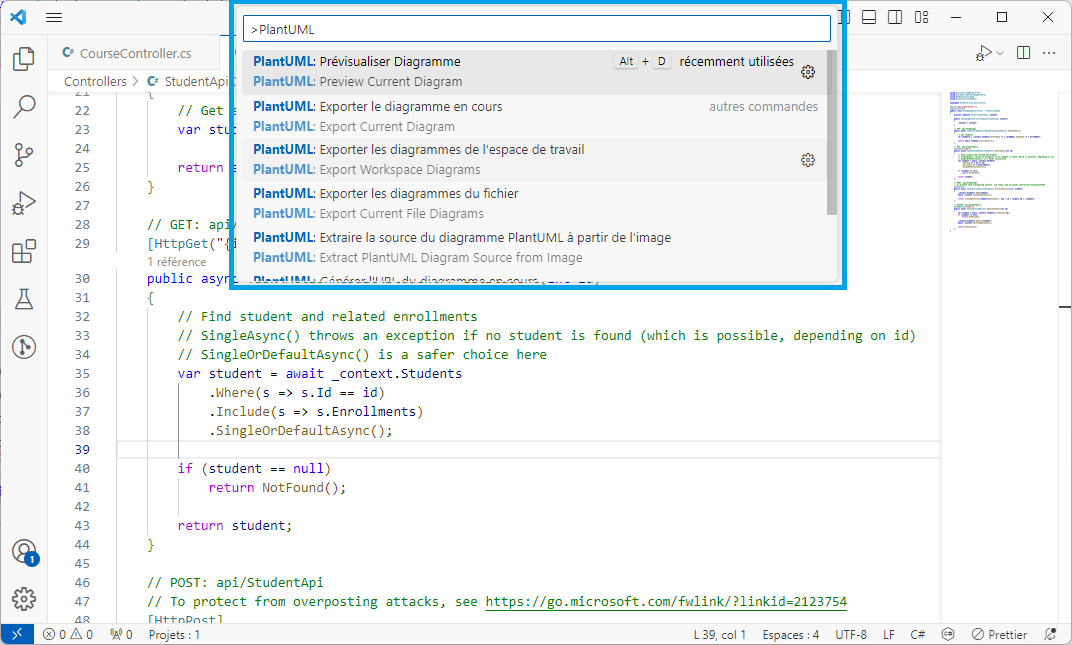
\includegraphics[height=0.4\linewidth]{figures/environnement/commande-ultime}
\end{frame}


\subsection{Le débogage}
\label{subsec:debogage}

\begin{frame}
    \frametitle{Les erreurs de compilation}
    \centering
    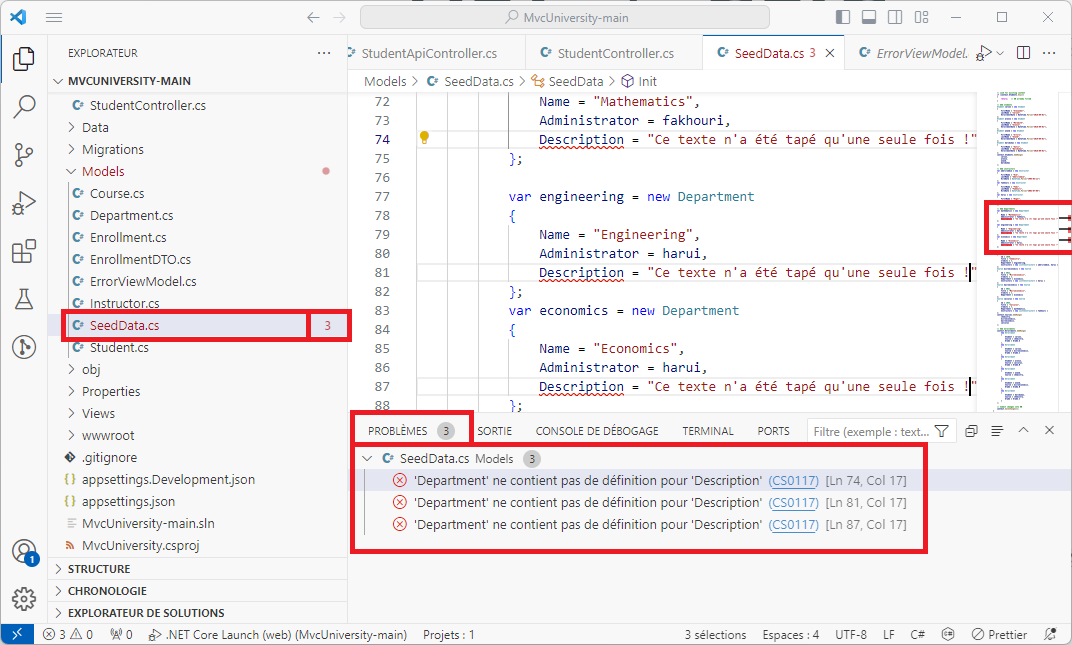
\includegraphics[height=0.5\linewidth]{figures/environnement/erreurs-de-compilation}
\end{frame}

\begin{frame}
    \frametitle{Poser un point d'arrêt}
    \centering
    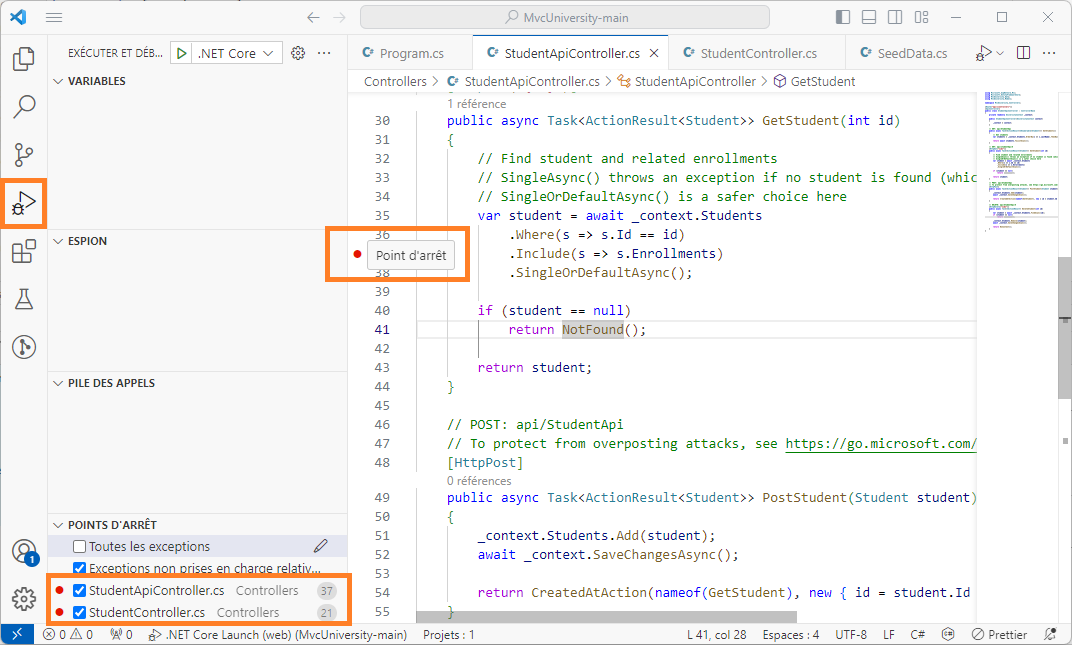
\includegraphics[height=0.5\linewidth]{figures/environnement/point-arret}
\end{frame}

\begin{frame}
    \frametitle{Lancement avec l'environnement de développement}
    \centering
    \Huge
    \textbf{F5}

    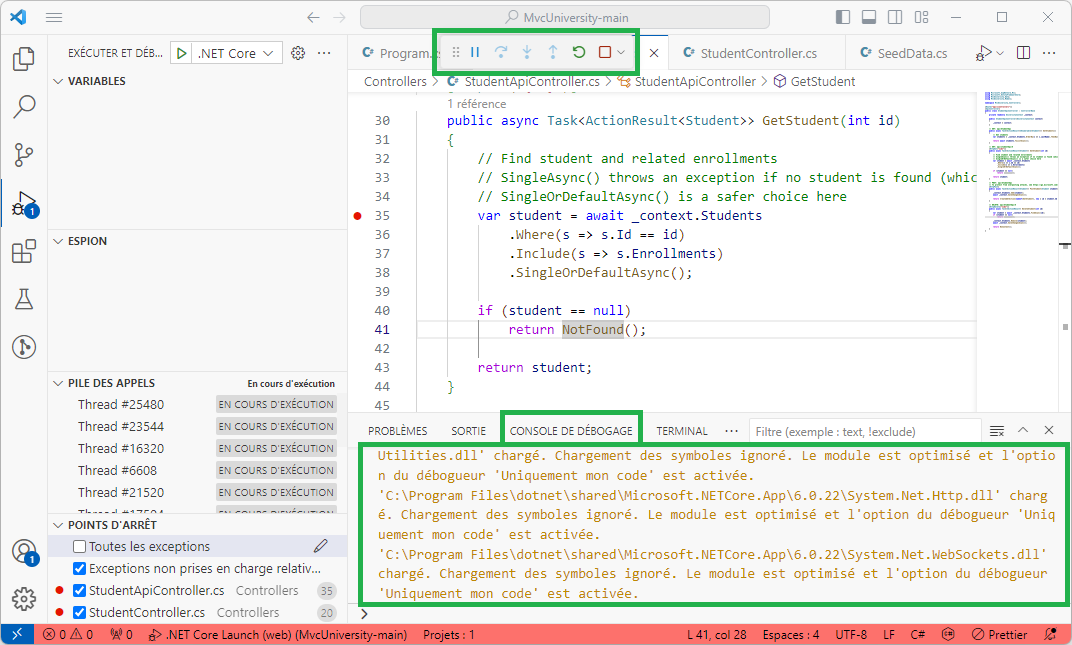
\includegraphics[height=0.4\linewidth]{figures/environnement/lancement-du-programme}
\end{frame}

\begin{frame}
    \frametitle{Examiner l'état du programme au point d'arrêt}
    \centering
    \includegraphics[height=0.5\linewidth]{figures/environnement/déboguage}
\end{frame}

\begin{frame}
    \frametitle{La pile d'exécution}
    \centering
    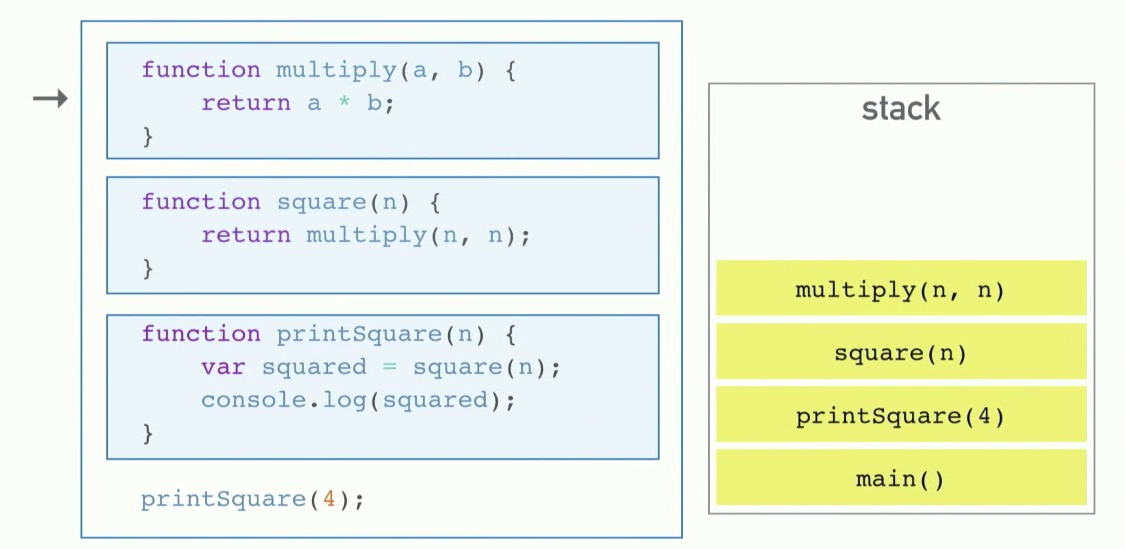
\includegraphics[height=0.5\linewidth]{figures/environnement/callstack}
\end{frame}

\begin{frame}
    \frametitle{La trace d'appels}
    \centering
    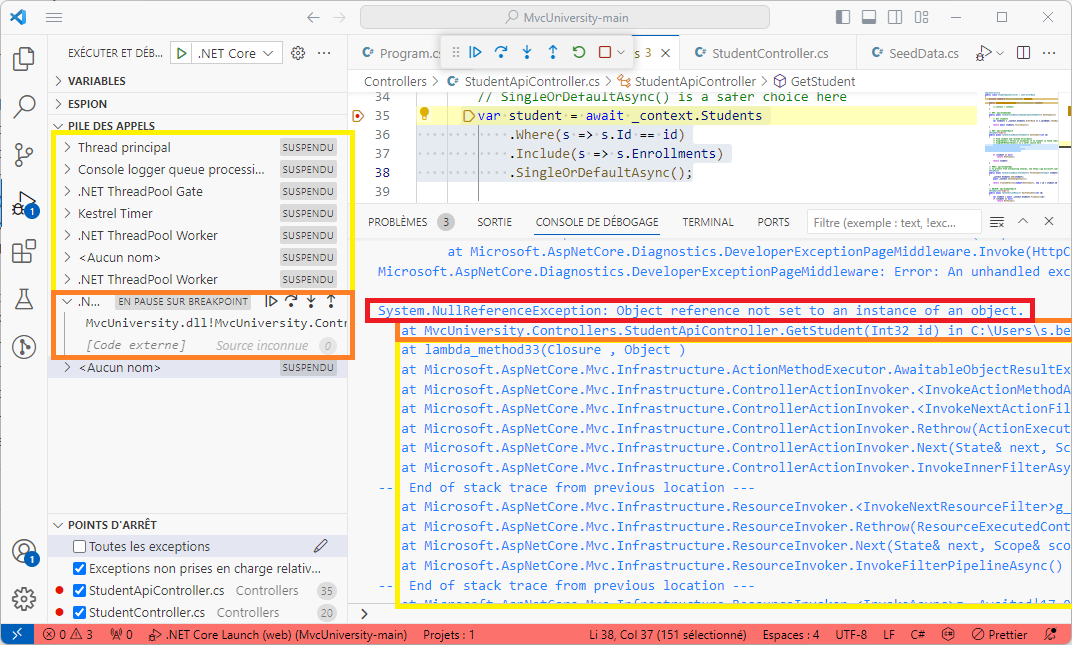
\includegraphics[height=0.5\linewidth]{figures/environnement/stacktrace}
\end{frame}

% debug, stacktrace,

\subsection{Gestion de version}
\label{subsec:cvs}

\begin{frame}
    \frametitle{Git}

    \emph{A silly, incompetent, stupid or annoying person (usually a man).}

    \textbf{Torvalds} sarcastically quipped about the name git:
    \enquote{I'm an egotistical bastard, and I name all my projects after myself. First 'Linux', now 'git'.}

    \enquote{git} can mean anything, depending on your mood.
    \begin{itemize}
        \item Random three-letter combination that is pronounceable, and not actually used by any common UNIX command ;
        \item \enquote{Global information tracker} ;
        \item \enquote{Goddamn idiotic truckload of sh*t} ;
    \end{itemize}

    The source code for Git refers to the program as \enquote{the information manager from hell}.
\end{frame}

\begin{frame}[fragile]
    \frametitle{Initialiser Git}

    \begin{lstlisting}[language=bash]
git config --global user.name "Your Name"
git config --global user.email "youremail@yourdomain.com"
    \end{lstlisting}

    \begin{center}
        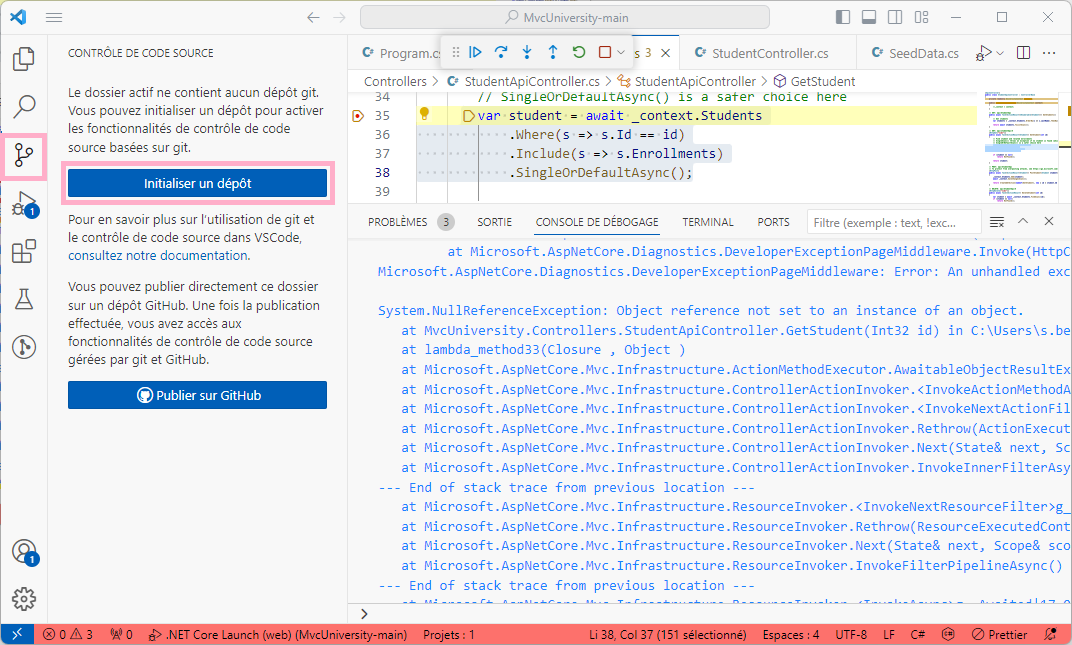
\includegraphics[height=0.4\linewidth]{figures/environnement/git-init}
    \end{center}
\end{frame}

\begin{frame}
    \frametitle{Valider \underline{régulièrement} les changements}
    \centering
    \begin{columns}
        \begin{column}{0.35\textwidth}
            \begin{enumerate}
                \item Écrire un peu de code ;
                \item Vérifier le résultat ;
                \item Valider les modifications.
            \end{enumerate}
        \end{column}
        \begin{column}{0.65\textwidth}
            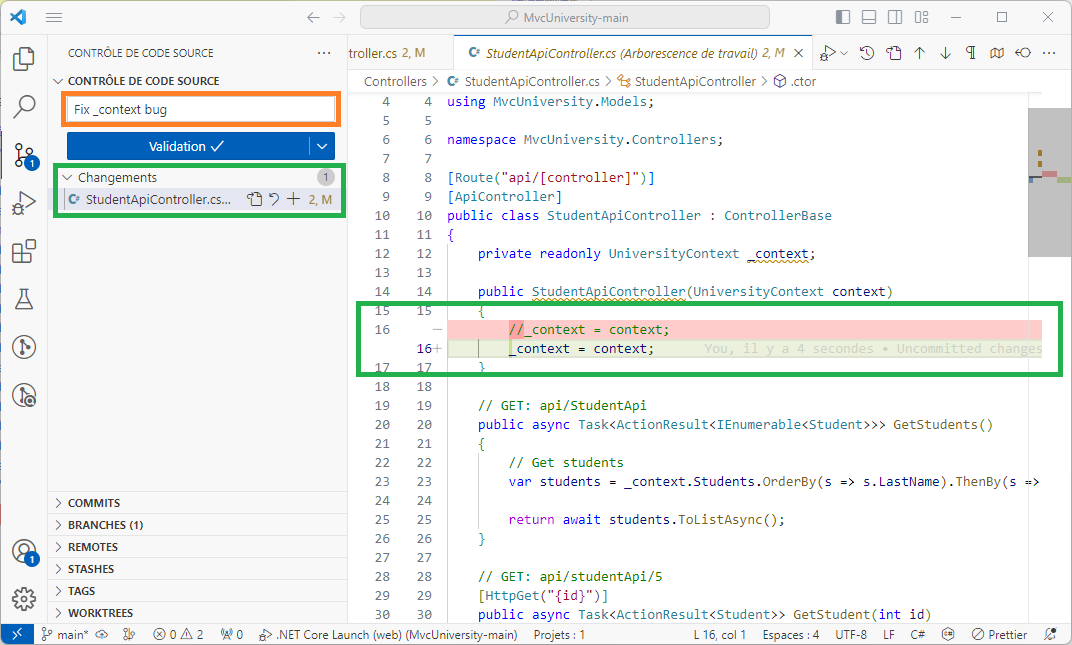
\includegraphics[width=\linewidth]{figures/environnement/git-commit}
        \end{column}
    \end{columns}
\end{frame}

\begin{frame}
    \frametitle{Les bases}
    \centering
    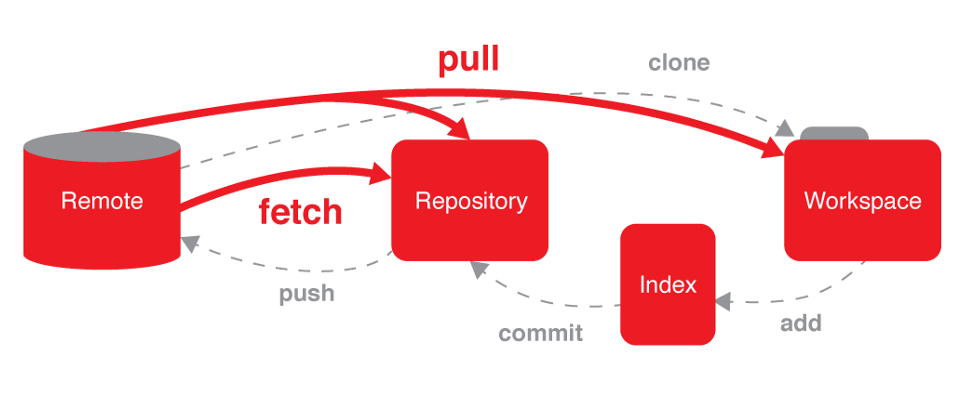
\includegraphics[width=\linewidth]{figures/environnement/git-spaces}
\end{frame}

\begin{frame}
    \frametitle{Les espaces}
    \begin{itemize}
        \item La remise (stash) : Un endroit où remiser des modifications pendant que vous travaillez sur autre chose.
        \item L'espace de travail : Votre dossier de travail !
        \item L'index : L'index (ou \enquote{zone de transit}) maintient un instantané de l'espace de travail qui servira de base pour le prochain commit.
        \item Le dépôt local : Un sous-répertoire nommé \textbf{.git} qui contient tous les fichiers nécessaires au référentiel.
        \item Le(s) dépôt(s) distant(s) : Versions de votre projet qui sont hébergés sur le réseau ou Internet, pour mettre toutes vos modifications à la disposition d'autres développeurs.
    \end{itemize}
\end{frame}

\begin{frame}
    \frametitle{Liste des commandes de l'espace de travail}
    \centering
    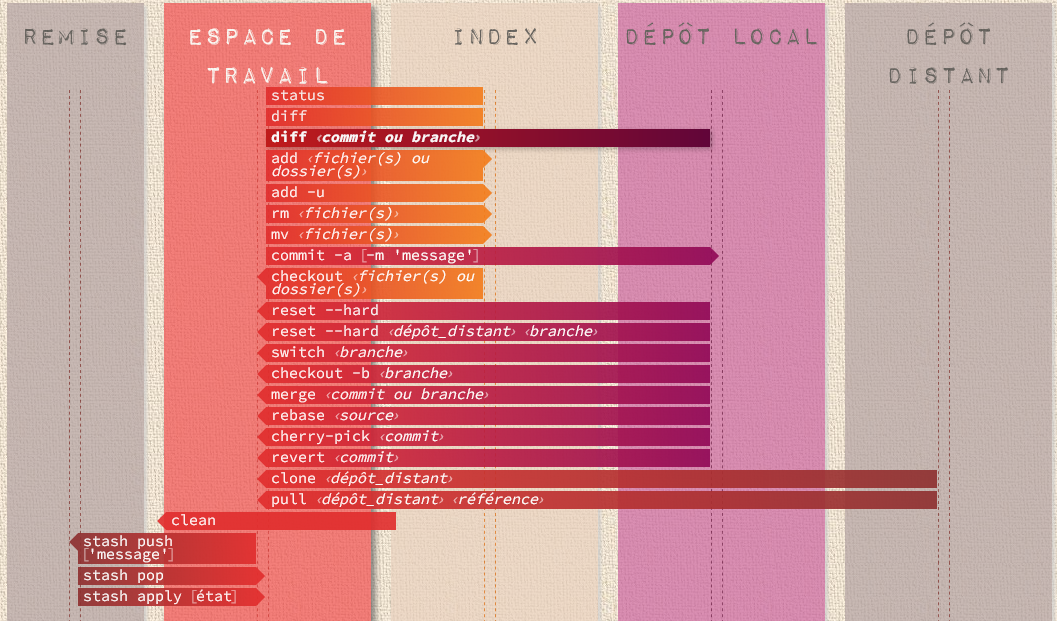
\includegraphics[height=0.5\linewidth]{figures/environnement/git-workspace}
\end{frame}

\begin{frame}
    \frametitle{Liste des commandes du dépôt local}
    \centering
    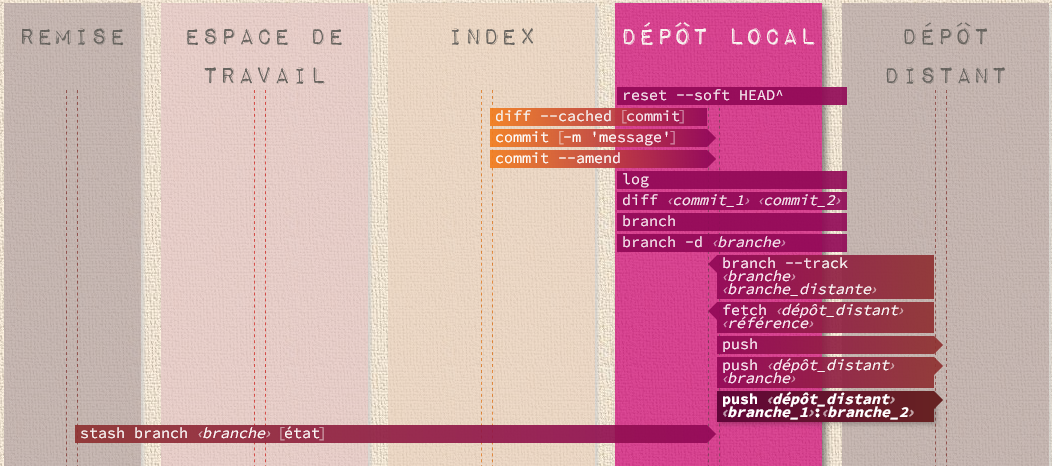
\includegraphics[width=\linewidth]{figures/environnement/git-local-repo}
\end{frame}

\begin{frame}
    \frametitle{Git Cheatsheet}
    \centering

    \qrcode[height=150pt]{https://ndpsoftware.com/git-cheatsheet.html\#loc=workspace;}
\end{frame}

\begin{frame}
    \frametitle{Modèle de branchement -- GitFlow}
    \centering
    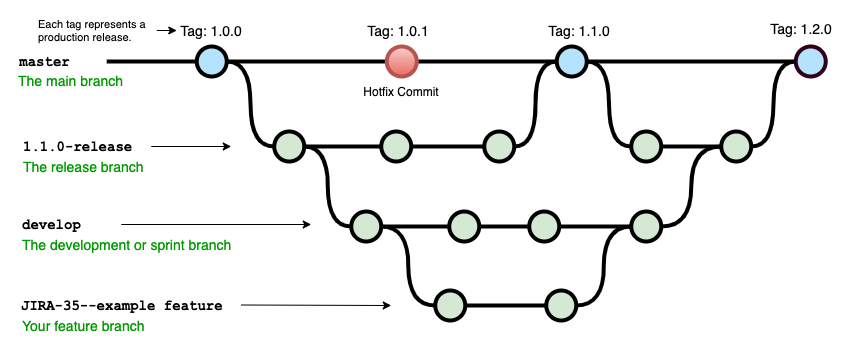
\includegraphics[width=\linewidth]{figures/environnement/git-branching-gitflow}
\end{frame}

\begin{frame}
    \frametitle{Modèle de branchement -- OneFlow}
    \centering
    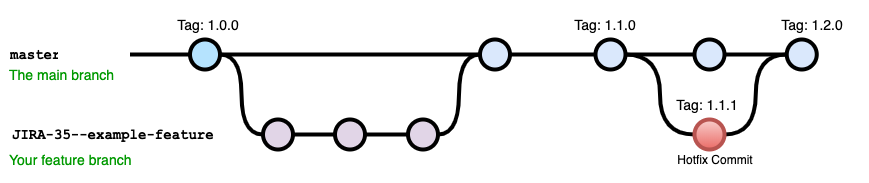
\includegraphics[width=\linewidth]{figures/environnement/git-branching-oneflow}
\end{frame}

\begin{frame}
    \frametitle{Modèle de branchement -- NoFlow (SVN)}
    \centering
    
\includegraphics[width=0.7\linewidth]{figures/environnement/git-branching-noflow}
\end{frame}

\begin{frame}
    \frametitle{Une extension pour Git}
    \centering
    \normalsize Installer l'extension VSCode : \texttt{ext install eamodio.gitlens} (CTRL+P)

    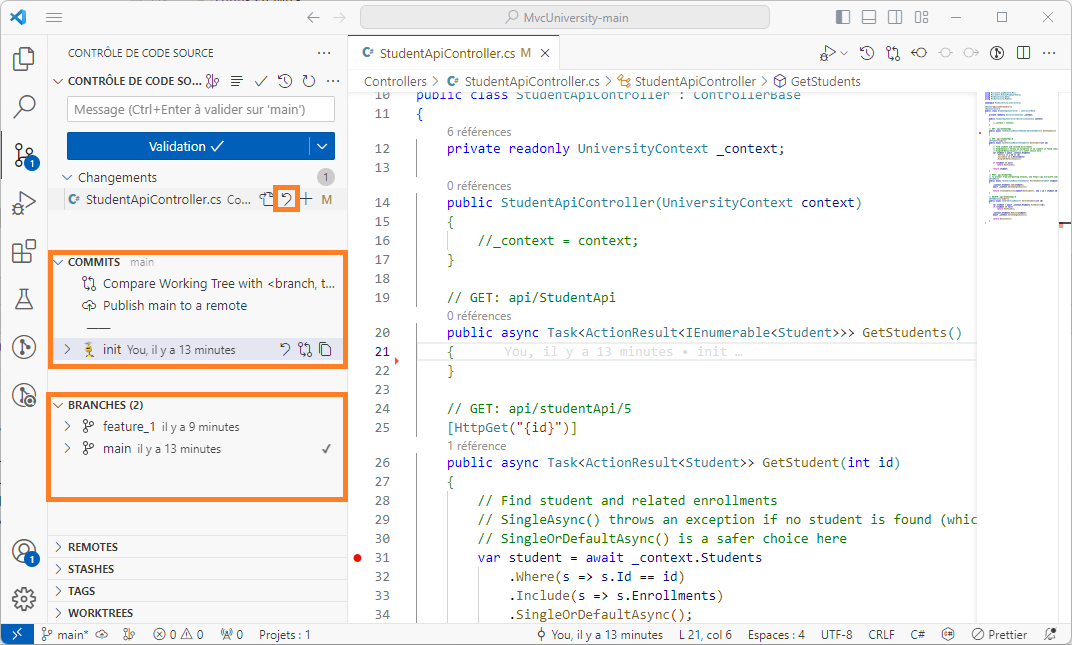
\includegraphics[height=0.4\linewidth]{figures/environnement/git-lens}
\end{frame}
